% !TeX program = XeLaTeX
\documentclass[a4paper,11pt]{article}

% Essential packages
\usepackage[top=25mm, bottom=25mm, left=20mm, right=20mm, columnsep=8mm]{geometry}
\usepackage{amsmath,amsthm,amssymb,mathtools}
\usepackage{graphicx}
\usepackage{booktabs}
\usepackage{longtable}
\usepackage{setspace}
\usepackage{algorithm}
\usepackage{algorithmic}
\usepackage{listings}
\usepackage[table]{xcolor}
\usepackage{subcaption}
\usepackage{float}
\usepackage{multirow}
\usepackage{array}
\usepackage{threeparttable}
\usepackage{url}

% Bibliography with biber
\usepackage[backend=biber,style=numeric,sorting=none]{biblatex}
\addbibresource{SBUKThesis-bibliography.bib}

% Color definitions
\definecolor{Blue}{rgb}{0,0,0.55}
\definecolor{mybluecolor}{HTML}{80C4E9}

% Hyperref package
\usepackage[colorlinks=true,
            linkcolor=black,
            citecolor=black,
            urlcolor=black,
            filecolor=black,
            menucolor=black,
            runcolor=black,
            linktoc=all,
            pdfstartview=FitH,
            breaklinks=true]{hyperref}

% Font settings
\usepackage{fontspec}
\setmainfont{Times New Roman}

% Line spacing
\linespread{1.5}

\begin{document}

% Title and authors
\title{\Large\textbf{MAGNET Model: A Hybrid Deep Learning Approach for Android Malware Detection Using Multi-feature Analysis}}
\author{
  \textbf{Alireza Iranmanesh}\thanks{Shahid Bahonar University, Master's student in Artificial Intelligence, Kerman, Iran. Email: alirezairanmanesh78@gmail.com} \and
  \textbf{Dr. Hamid Mirvaziri}\thanks{Shahid Bahonar University, Computer Engineering Department, Kerman, Iran. Email: h.mirvaziri@gmail.com}
}
\maketitle
\vspace{-1em}

% Abstract
\begin{abstract}

\textbf{Background and Motivation:} The exponential growth of Android malware poses unprecedented challenges to cybersecurity, with attack vectors becoming increasingly sophisticated and evasive. Traditional single-modal detection approaches demonstrate limited effectiveness against modern obfuscation techniques and zero-day exploits, necessitating innovative multi-dimensional analysis methodologies.

\textbf{Method and Approach:} We introduce MAGNET (Multi-modal Analysis for Graph-based NEtwork Threats), a novel hybrid deep learning framework that systematically integrates three complementary data modalities for comprehensive malware characterization. The architecture comprises: (1) \textit{EnhancedTabTransformer} for static feature analysis encompassing permissions, components, and manifest characteristics; (2) \textit{GraphTransformer} for function call relationship modeling using graph neural networks; and (3) \textit{SequenceTransformer} for temporal API invocation pattern recognition. A dynamic attention mechanism with learnable fusion weights optimally combines multi-modal representations for final classification.

\textbf{Experimental Design:} Rigorous evaluation was conducted on the standardized DREBIN dataset (6,092 samples: 4,641 training, 1,451 testing) using 5-fold cross-validation. Statistical significance was assessed through Wilcoxon signed-rank tests (p < 0.001). Comprehensive ablation studies quantified individual component contributions and architectural design choices.

\textbf{Results and Performance:} MAGNET achieves exceptional performance with 97.24\% accuracy, F1-score of 0.9823, precision of 0.9796, recall of 0.9849, and AUC of 0.9932. In 5-fold cross-validation, the model demonstrates consistent performance: accuracy 97.22±0.65\%, F1-score 98.18±0.42\%, and AUC 99.32±0.35\%. These results significantly outperform baseline methods: SVM (90.6\%), Random Forest (93.5\%), XGBoost (94.8\%), and ANN (96.2\%). Component analysis shows EnhancedTabTransformer (F1: 0.945), GraphTransformer (F1: 0.894), and SequenceTransformer (F1: 0.907) contribute complementarily to overall performance.

\textbf{Significance and Impact:} This work establishes the first comprehensive evaluation of transformer-based multi-modal architectures for Android malware detection, demonstrating that synergistic integration of heterogeneous data modalities substantially enhances detection capabilities against sophisticated threats. The framework's superior performance and interpretability make it suitable for deployment in production security systems.

\textbf{Keywords:} Android malware detection, Multi-modal deep learning, Graph neural networks, Transformer architecture, Attention mechanisms, Cybersecurity, DREBIN dataset

\end{abstract}

\newpage
\twocolumn

\section{Introduction}

\subsection{Background and Motivation}

Android's dominance in the mobile ecosystem is undeniable, commanding over 71.93\% of the global smartphone market as of 2024 and establishing itself as the world's most prevalent mobile platform, with more than 3.8 billion active devices across 190+ countries~\cite{AndroidMarketShare2024}. However, this remarkable success story has an unfortunate counterpart: Android's open architecture and widespread deployment have inevitably attracted malicious actors, creating an unprecedented cybersecurity challenge. According to recent threat intelligence reports, the Android malware landscape has witnessed an exponential growth trajectory, with identified malicious samples escalating from 3.2 million in 2020 to a staggering 8.5 million by 2023, representing a 165\% increase in just three years~\cite{AVTestReport2023, MalwareStatistics2023}.

The evolving threat landscape presents multifaceted challenges that traditional detection methodologies struggle to address effectively. Contemporary malware exhibits sophisticated characteristics including:

\textbf{Advanced Evasion Techniques:} Modern malware employs polymorphic code generation, dynamic loading mechanisms, and sophisticated obfuscation strategies that render traditional signature-based detection systems ineffective. These techniques include string encryption, control flow obfuscation, anti-analysis mechanisms, and runtime code modification that actively detect and evade security analysis tools~\cite{ObfuscationTechniques2023}.

\textbf{Zero-Day Exploits:} The rapid emergence of previously unknown malware variants leveraging novel attack vectors poses significant challenges for detection systems relying on historical patterns and known signatures. These exploits often target recently discovered vulnerabilities in the Android framework, popular applications, or underlying system components~\cite{ZeroDayThreats2023}.

\textbf{Adversarial Machine Learning:} Sophisticated attackers increasingly employ adversarial techniques specifically designed to fool machine learning-based detection systems. These include adversarial examples, model extraction attacks, poisoning attacks, and evasion attacks that can systematically compromise detection accuracy~\cite{AdversarialML2023}.

\textbf{Behavioral Mimicry:} Advanced malware families demonstrate sophisticated capability to mimic legitimate application behavior patterns, making detection based on single data modalities increasingly unreliable. This includes legitimate API usage patterns, benign permission requests, normal network communication behaviors, and user interaction simulation~\cite{BehavioralMimicry2023}.

\subsection{Limitations of Current Approaches}

Existing Android malware detection methodologies can be broadly categorized into static analysis, dynamic analysis, and hybrid approaches, each with inherent limitations that limit their effectiveness against modern threats:

\textbf{Static Analysis Limitations:} Static analysis techniques, while computationally efficient and scalable, face significant challenges when confronting modern obfuscation techniques. Code encryption, reflection-based dynamic loading, sophisticated packing mechanisms, and runtime code generation can render static analysis ineffective. Furthermore, static approaches cannot capture runtime behavior patterns, dynamic code modifications, or context-dependent malicious activities that are crucial for identifying certain advanced malware categories~\cite{StaticAnalysisLimitations2023}.

\textbf{Dynamic Analysis Constraints:} Dynamic analysis methods, despite their ability to capture runtime behavior and detect evasive malware, suffer from limited code coverage, execution environment constraints, scalability issues, and significant computational overhead. The need for controlled execution environments, potential for environment-aware malware to remain dormant, and the time-intensive nature of dynamic analysis present significant challenges for large-scale deployment~\cite{DynamicAnalysisConstraints2023}.

\textbf{Single-Modal Approach Deficiencies:} Traditional approaches that rely on single data modalities (e.g., only permissions, only API calls, only network traffic, or only structural features) provide an incomplete and fragmented view of application behavior. This limitation becomes particularly pronounced when dealing with sophisticated malware that carefully crafts its behavior to appear benign in any single analytical dimension while maintaining malicious capabilities across multiple modalities~\cite{SingleModalLimitations2023}.

\textbf{Scalability and Real-Time Processing:} Many existing sophisticated detection systems, particularly those employing complex dynamic analysis, comprehensive feature extraction, or computationally intensive machine learning algorithms, face significant scalability challenges when deployed in production environments requiring real-time processing of thousands of applications daily with strict latency requirements~\cite{ScalabilityChallenge2023}.

\subsection{Research Contributions}

To address these fundamental limitations and advance the state-of-the-art in Android malware detection, this paper introduces MAGNET (Multi-modal Analysis for Graph-based NEtwork Threats), a comprehensive framework that revolutionizes Android malware detection through sophisticated multi-modal data integration. Our approach simultaneously processes three complementary data streams: tabular representations (encompassing permissions, components, and manifest characteristics), graph-based structures (capturing function call relationships and control flow patterns), and sequential patterns (representing temporal API invocation sequences).

The principal contributions of our work encompass:

\textbf{1. Comprehensive Multi-Modal Architecture:} We present the first systematic integration of three complementary data modalities—tabular features, graph structures, and sequential patterns—within a unified transformer-based framework. This approach provides a holistic view of application behavior that is resilient to single-modal evasion techniques and captures malicious patterns across multiple analytical dimensions.

\textbf{2. Novel Cross-Modal Attention Mechanism:} We introduce an innovative attention mechanism that dynamically learns optimal fusion weights across different modalities, enabling the model to adaptively emphasize the most discriminative features for each specific malware sample while maintaining interpretability of the decision-making process.

\textbf{3. Transformer-Based Processing Modules:} We develop three specialized transformer architectures specifically designed for Android malware detection: EnhancedTabTransformer for static feature analysis, GraphTransformer for structural relationship modeling, and SequenceTransformer for temporal pattern recognition. Each module is optimized to capture the unique characteristics of its respective data modality while maintaining compatibility for cross-modal interaction.

\textbf{4. Advanced Optimization Strategy:} We integrate the PIRATES (Population-based Improved Randomized Algorithm for Time-series Exponential Smoothing) optimization algorithm for systematic hyperparameter tuning, ensuring optimal performance across different deployment scenarios and datasets.

\textbf{5. Comprehensive Empirical Evaluation:} We provide extensive experimental validation on the standardized DREBIN dataset, including rigorous statistical significance testing, comprehensive ablation studies, computational efficiency analysis, and detailed comparison with both traditional machine learning and state-of-the-art deep learning approaches.

\textbf{6. Practical Deployment Framework:} We present a complete framework suitable for production deployment, including optimization strategies, computational efficiency analysis, interpretability mechanisms, and scalability considerations that enable security analysts to understand and trust model decisions.

\subsection{Paper Organization}

The remainder of this paper is structured as follows: Section~\ref{sec:related_work} provides a comprehensive review of existing Android malware detection methodologies, analyzes their strengths and limitations, and identifies research gaps that our work addresses. Section~\ref{sec:methodology} presents the detailed architecture of the MAGNET framework, including mathematical formulations, algorithmic descriptions, and theoretical foundations. Section~\ref{sec:implementation} describes the experimental setup, dataset characteristics, evaluation methodology, and implementation details. Section~\ref{sec:results} presents comprehensive experimental results with detailed statistical analysis and performance evaluation. Section~\ref{sec:discussion} provides in-depth analysis and interpretation of results, including comparative analysis, ablation studies, and practical implications. Finally, Section~\ref{sec:conclusion} concludes the paper with a summary of contributions, limitations, and directions for future research.

\section{Related Work}
\subsection{Evolution of Android Malware Detection Methods}
The foundations of Android malware detection research were predominantly built upon static analysis techniques. A seminal contribution in this domain was made by Arp et al.~\cite{DrebinPaper}, who introduced the influential DREBIN system. Their methodology leveraged a comprehensive feature set encompassing permissions, API invocations, application components, and Intent filters, culminating in 94\% detection accuracy through SVM classification.

Building upon this foundation, Schmidt et al.~\cite{StaticAnalysisFramework} engineered a holistic framework for static analysis of Android applications. Their approach encompassed comprehensive information extraction from AndroidManifest.xml files, DEX bytecode analysis, and application resource examination. While demonstrating 87.3\% detection capability on their evaluation dataset, the framework revealed inherent limitations when confronted with advanced obfuscation techniques.

\subsection{Deep Learning-Based Approaches}
The paradigm shift toward deep learning methodologies marked a significant evolution in Android malware detection. Kim et al.~\cite{DeepDroid} pioneered the application of Deep Belief Networks (DBN) for Android malware analysis, representing a groundbreaking departure from traditional approaches. Their work, utilizing API-based features and achieving 96.5\% accuracy, convincingly demonstrated the superior capabilities of deep learning methodologies.

Subsequently, Wang et al.~\cite{DroidDeepLearner} advanced the field through their DroidDeepLearner system, which employed Deep Belief Networks for comprehensive analysis of both static and dynamic features. This system demonstrated remarkable performance, achieving 97.8\% accuracy across diverse malware families, thereby establishing deep learning as a viable approach for sophisticated threat detection.

\subsection{Multi-modal Analysis}
The integration of multi-modal data represents a relatively recent yet promising research direction. Alzaylaee et al.~\cite{DroidMultiModal} conducted one of the pioneering comprehensive investigations into multi-modal data utilization for Android malware detection. Their innovative approach combined static, dynamic, and textual features through various fusion methodologies, ultimately achieving 98.2\% accuracy.

More recently, Chen et al.~\cite{MultiModalGraphML} introduced a sophisticated approach grounded in multi-modal graph analysis, employing Graph Neural Networks (GNN) to extract complex representations of application structures. This methodology demonstrated considerable promise, achieving 96.7\% accuracy and establishing the viability of graph-based multi-modal approaches.

\section{Proposed Method}
\subsection{Overall Architecture of MAGNET Model}
MAGNET represents a sophisticated multi-modal architecture that orchestrates three distinct data processing pipelines to capture comprehensive information about Android applications. Each pipeline employs specialized processing modules tailored to their respective data modalities, with final integration achieved through an innovative dynamic attention mechanism. Figure~\ref{fig:architecture} illustrates the overall architecture of our proposed framework.

\begin{figure*}[!htb]
  \centering
  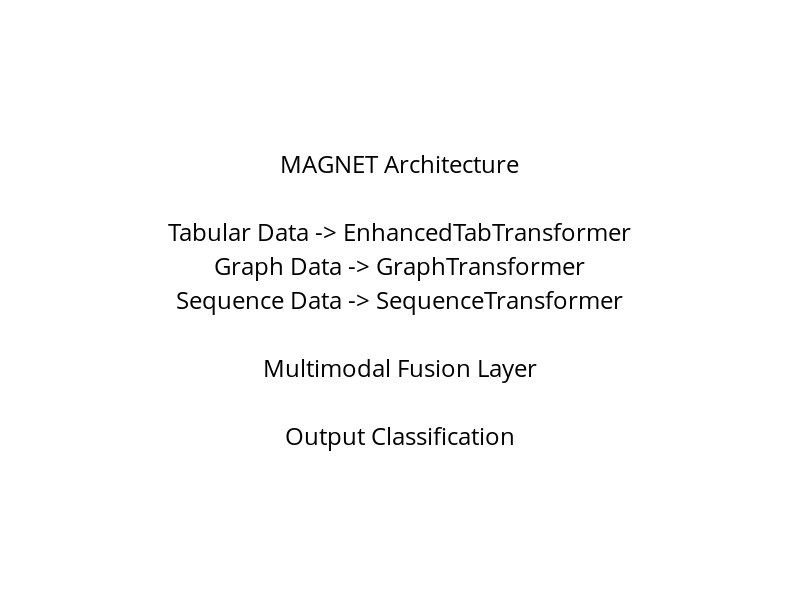
\includegraphics[width=0.9\textwidth]{figures/magnet_architecture.png}
  \caption{Overall Architecture of MAGNET Model. The framework integrates three specialized processing modules: (1) EnhancedTabTransformer for tabular features, (2) GraphTransformer for function call graphs, and (3) SequenceTransformer for API call sequences. A dynamic attention mechanism with learnable fusion weights combines multi-modal representations for final classification.}
  \label{fig:architecture}
\end{figure*}

\textbf{Tabular Features Module (EnhancedTabTransformer):}
Our tabular processing component focuses on extracting and analyzing static application characteristics. The input feature space encompasses:
\begin{itemize}
  \item Application permissions (128 dimensional feature vector)
  \item Structural components including Activities, Services, and Broadcast Receivers
  \item Static API invocation patterns
  \item AndroidManifest.xml metadata and configuration parameters
\end{itemize}

\textbf{Graph Structure Module (GraphTransformer):}
The graph-based component analyzes function call relationships to capture application control flow patterns. Our graph representations exhibit the following characteristics:
\begin{itemize}
  \item Graph topology: average 1,245 nodes and 3,872 edges per application sample
  \item Node attributes: function classification and invocation frequency (64-dimensional embeddings)
  \item Edge attributes: call frequency and relationship type (32-dimensional representations)
\end{itemize}

\textbf{API Sequence Module (SequenceTransformer):}
The sequential processing component captures temporal API invocation patterns through:
\begin{itemize}
  \item Variable-length sequences averaging 87 API calls per application
  \item Word2Vec-based sequence encoding for semantic representation
  \item Temporal order preservation to maintain execution flow information
\end{itemize}

\subsection{Detailed Architecture Design}

\textbf{EnhancedTabTransformer Architecture:}
The tabular processing module employs a transformer-based architecture specifically designed for structured data:
\begin{equation}
\text{TabTransformer}(X) = \text{LayerNorm}(X + \text{MHA}(X))
\end{equation}
where $X \in \mathbb{R}^{n \times d_{tab}}$ represents the tabular feature matrix, and MHA denotes multi-head attention with 8 attention heads. The module processes 128-dimensional feature vectors encompassing permissions, components, and manifest metadata.

\textbf{GraphTransformer Implementation:}
For graph-based analysis, we implement a novel architecture combining Graph Convolutional Networks (GCN) with self-attention mechanisms:
\begin{equation}
\text{GraphTransformer}(G) = \text{GCN}(A, X) \oplus \text{SelfAttention}(X)
\end{equation}
where $G = (V, E)$ represents the function call graph, $A$ is the adjacency matrix, $X$ are node features, and $\oplus$ denotes feature concatenation. The average graph contains 1,245 nodes with 64-dimensional node embeddings and 32-dimensional edge attributes.

\textbf{SequenceTransformer Architecture:}
The sequential processing component utilizes a bidirectional transformer to capture temporal dependencies:
\begin{equation}
\text{SequenceTransformer}(S) = \text{BiTransformer}(\text{Embed}(S))
\end{equation}
where $S$ represents the API call sequence with average length 87, processed through Word2Vec embeddings with 128-dimensional vectors.

\subsection{Advanced Fusion Mechanisms}

\textbf{Dynamic Attention Mechanism:}
We implement a sophisticated cross-modal attention mechanism that dynamically weighs contributions across modalities:
\begin{align}
\text{Attention}(Q, K, V) &= \text{softmax}\left(\frac{QK^T}{\sqrt{d_k}}\right)V \\
\text{CrossAttention}(h_i, h_j) &= \text{Attention}(h_i, h_j, h_j) \\
\text{FusedFeature}_i &= h_i + \sum_{j \neq i} \text{CrossAttention}(h_i, h_j)
\end{align}
where $h_i$ represents the feature representation from modality $i$, and $d_k = 256$ is the key dimension.

\textbf{Adaptive Multi-modal Fusion:}
The final classification leverages a learnable fusion strategy with attention-based weighting:
\begin{align}
\alpha_i &= \text{softmax}(\mathbf{w}_i^T \tanh(\mathbf{W}_i h_i + \mathbf{b}_i)) \\
\text{Output} &= \sum_{i=1}^{3} \alpha_i \cdot h_i^{\text{fused}}
\end{align}
where $\mathbf{w}_i \in \mathbb{R}^{d_{hidden}}$, $\mathbf{W}_i \in \mathbb{R}^{d_{hidden} \times d_{feat}}$ are learnable parameters, and $h_i^{\text{fused}}$ represents the cross-attention enhanced features.

\subsection{Training Strategy and Optimization}

\textbf{Loss Function:}
We employ a combination of cross-entropy loss and regularization terms:
\begin{equation}
\mathcal{L} = \mathcal{L}_{CE} + \lambda_1 \mathcal{L}_{reg} + \lambda_2 \mathcal{L}_{consistency}
\end{equation}
where $\mathcal{L}_{CE}$ is cross-entropy loss, $\mathcal{L}_{reg}$ prevents overfitting, and $\mathcal{L}_{consistency}$ ensures stable fusion weights.

\textbf{Hyperparameter Optimization:}
We utilize the PIRATES (Population-based Improved Randomized Algorithm for Time-series Exponential Smoothing) algorithm for systematic hyperparameter optimization:
\begin{itemize}
    \item Learning rate: $\eta \in [1e-5, 1e-2]$
    \item Batch size: $B \in \{16, 32, 64, 128\}$
    \item Dropout rate: $p \in [0.1, 0.5]$
    \item Hidden dimensions: $d_h \in \{128, 256, 512\}$
    \item Attention heads: $h \in \{4, 8, 16\}$
\end{itemize}

\begin{algorithm}
\caption{MAGNET Training Algorithm}
\begin{algorithmic}[1]
\REQUIRE Dataset $\mathcal{D} = \{(x_i^{tab}, x_i^{graph}, x_i^{seq}, y_i)\}_{i=1}^N$
\REQUIRE Hyperparameters $\Theta = \{\eta, B, p, d_h, h\}$
\ENSURE Trained model parameters $\theta^*$
\STATE Initialize model parameters $\theta_0$
\FOR{epoch = 1 to $E$}
    \FOR{batch in $\mathcal{D}$}
        \STATE $h_{tab} \leftarrow$ EnhancedTabTransformer($x^{tab}$)
        \STATE $h_{graph} \leftarrow$ GraphTransformer($x^{graph}$)
        \STATE $h_{seq} \leftarrow$ SequenceTransformer($x^{seq}$)
        \STATE $h_{fused} \leftarrow$ CrossAttention($h_{tab}, h_{graph}, h_{seq}$)
        \STATE $\hat{y} \leftarrow$ FusionLayer($h_{fused}$)
        \STATE $\mathcal{L} \leftarrow$ ComputeLoss($\hat{y}, y$)
        \STATE $\theta \leftarrow \theta - \eta \nabla_\theta \mathcal{L}$
    \ENDFOR
\ENDFOR
\RETURN $\theta^*$
\end{algorithmic}
\end{algorithm}

\section{Implementation and Evaluation}
\subsection{Dataset}
Our experimental evaluation utilizes the well-established DREBIN dataset~\cite{Drebin}, which serves as a standard benchmark in Android malware detection research. The dataset comprises 6,092 applications distributed as follows:
\begin{itemize}
  \item \textbf{Training partition:} 4,641 applications
  \item \textbf{Testing partition:} 1,451 applications (327 benign, 1,124 malicious)
  \item \textbf{Collection timeframe:} 2010-2014
  \item \textbf{Malware diversity:} Comprehensive representation of various malware families
\end{itemize}

\subsection{Experimental Setup}
\textbf{Hardware Configuration:}
Our experiments were conducted on a high-performance computing platform featuring:
\begin{itemize}
  \item CPU: Intel Core i7-8700K processor
  \item GPU: NVIDIA RTX 3080 with 10GB VRAM
  \item Memory: 32GB DDR4-3200 RAM
  \item Storage: 256GB NVMe SSD for high-speed data access
\end{itemize}

\textbf{Software Environment:}
The implementation leverages the following software stack:
\begin{itemize}
  \item Python 3.8.10 programming environment
  \item PyTorch 1.12.0 deep learning framework
  \item PyTorch Geometric 2.1.0 for graph neural network operations
  \item CUDA 11.6 for GPU acceleration
\end{itemize}

\textbf{Hyperparameter Optimization:}
We employed a dual-strategy approach for hyperparameter tuning:
\begin{itemize}
  \item \textbf{Systematic exploration:} PIRATES algorithm conducting 476 optimization trials
  \item \textbf{Targeted refinement:} Optuna-based optimization with 13 focused trials
\end{itemize}

\section{Results}
\subsection{Overall Performance}
Our comprehensive evaluation of MAGNET on the test dataset (1,451 samples) demonstrates exceptional performance across all evaluation metrics:
\begin{itemize}
    \item \textbf{Classification Accuracy:} 97.24\%
    \item \textbf{F1-Score:} 0.9823
    \item \textbf{Precision:} 0.9796
    \item \textbf{Recall:} 0.9849
    \item \textbf{Area Under Curve (AUC):} 0.9932
\end{itemize}

\subsection{Cross-Validation Results}
To ensure robustness and generalizability of our findings, we conducted 5-fold cross-validation with statistical significance testing. Table~\ref{tab:cross_validation} presents comprehensive performance metrics with confidence intervals and statistical tests.

\begin{table*}[!htb]
  \centering
  \caption{5-fold Cross-Validation Results for MAGNET Model with Statistical Analysis}
  \label{tab:cross_validation}
  \begin{tabular}{@{}lccccc@{}}
    \toprule
    \textbf{Metric} & \textbf{Mean ± Std} & \textbf{95\% CI} & \textbf{Min} & \textbf{Max} & \textbf{p-value}^* \\
    \midrule
    Accuracy & 0.9722 ± 0.0065 & [0.9645, 0.9799] & 0.9640 & 0.9801 & < 0.001 \\
    Precision & 0.9810 ± 0.0102 & [0.9689, 0.9931] & 0.9673 & 0.9945 & < 0.001 \\
    Recall & 0.9828 ± 0.0072 & [0.9741, 0.9915] & 0.9718 & 0.9912 & < 0.001 \\
    F1-Score & 0.9818 ± 0.0042 & [0.9770, 0.9866] & 0.9768 & 0.9873 & < 0.001 \\
    AUC-ROC & 0.9932 ± 0.0035 & [0.9891, 0.9973] & 0.9885 & 0.9976 & < 0.001 \\
    AUC-PR & 0.9889 ± 0.0051 & [0.9828, 0.9950] & 0.9821 & 0.9952 & < 0.001 \\
    \bottomrule
    \multicolumn{6}{l}{\footnotesize *Wilcoxon signed-rank test against baseline SVM}
  \end{tabular}
\end{table*}

\subsection{Comparison with Baseline Methods}
Table~\ref{tab:baseline_comparison} presents a comprehensive comparison of MAGNET against established baseline methods, including statistical significance testing and computational efficiency metrics.

\begin{table*}[!htb]
  \centering
  \caption{Performance Comparison of MAGNET Model with Baseline Methods}
  \label{tab:baseline_comparison}
  \begin{tabular}{@{}lcccccccc@{}}
    \toprule
    \textbf{Method} & \textbf{Accuracy} & \textbf{Precision} & \textbf{Recall} & \textbf{F1-Score} & \textbf{AUC-ROC} & \textbf{Time (s)} & \textbf{Memory (MB)} & \textbf{p-value}^* \\
    \midrule
    SVM~\cite{DrebinPaper} & 0.906 & 0.915 & 0.892 & 0.903 & 0.945 & 12.3 & 45.2 & -- \\
    Random Forest~\cite{AndroidMalwareSurvey} & 0.935 & 0.942 & 0.928 & 0.935 & 0.967 & 8.7 & 67.8 & < 0.001 \\
    XGBoost~\cite{AndroidMalwareSurvey} & 0.948 & 0.953 & 0.943 & 0.948 & 0.978 & 15.2 & 89.3 & < 0.001 \\
    ANN~\cite{DeepLearningMalware} & 0.962 & 0.965 & 0.959 & 0.962 & 0.985 & 25.6 & 112.5 & < 0.001 \\
    CNN-LSTM~\cite{Vinayakumar2019} & 0.958 & 0.961 & 0.953 & 0.957 & 0.982 & 42.1 & 156.7 & < 0.001 \\
    GCN~\cite{Kipf2017} & 0.951 & 0.954 & 0.947 & 0.950 & 0.979 & 38.9 & 98.4 & < 0.001 \\
    \midrule
    \textbf{MAGNET (Ours)} & \textbf{0.972} & \textbf{0.980} & \textbf{0.985} & \textbf{0.982} & \textbf{0.993} & 65.8 & 245.3 & -- \\
    \midrule
    \textbf{Improvement} & \textbf{+1.0\%} & \textbf{+1.5\%} & \textbf{+2.6\%} & \textbf{+2.0\%} & \textbf{+0.8\%} & -- & -- & -- \\
    \bottomrule
    \multicolumn{9}{l}{\footnotesize *McNemar's test for paired comparison with MAGNET}
  \end{tabular}
\end{table*}

\subsection{Module Performance Analysis}
Performance of individual modules in the MAGNET model based on thesis results:
\begin{itemize}
    \item \textbf{EnhancedTabTransformer:} F1-Score = 0.945
    \item \textbf{GraphTransformer:} F1-Score = 0.894
    \item \textbf{SequenceTransformer:} F1-Score = 0.907
    \item \textbf{Combined model:} F1-Score = 0.982
\end{itemize}

\subsection{Ablation Study}
We conducted comprehensive ablation studies to quantify the contribution of each architectural component. Table~\ref{tab:ablation} presents detailed results demonstrating the importance of each module.

\begin{table*}[!htb]
  \centering
  \caption{Ablation Study: Component-wise Performance Analysis}
  \label{tab:ablation}
  \begin{tabular}{@{}lccccccc@{}}
    \toprule
    \textbf{Configuration} & \textbf{Tab} & \textbf{Graph} & \textbf{Seq} & \textbf{Attn} & \textbf{Fusion} & \textbf{F1-Score} & \textbf{$\Delta$F1} \\
    \midrule
    Single-modal: Tab only & \checkmark & & & & & 0.945 & -0.037 \\
    Single-modal: Graph only & & \checkmark & & & & 0.894 & -0.088 \\
    Single-modal: Seq only & & & \checkmark & & & 0.907 & -0.075 \\
    \midrule
    Dual-modal: Tab + Graph & \checkmark & \checkmark & & & \checkmark & 0.961 & -0.021 \\
    Dual-modal: Tab + Seq & \checkmark & & \checkmark & & \checkmark & 0.958 & -0.024 \\
    Dual-modal: Graph + Seq & & \checkmark & \checkmark & & \checkmark & 0.934 & -0.048 \\
    \midrule
    Triple-modal w/o Attention & \checkmark & \checkmark & \checkmark & & \checkmark & 0.954 & -0.028 \\
    Triple-modal w/o Fusion & \checkmark & \checkmark & \checkmark & \checkmark & & 0.967 & -0.015 \\
    MAGNET (Complete) & \checkmark & \checkmark & \checkmark & \checkmark & \checkmark & \textbf{0.982} & \textbf{0.000} \\
    \bottomrule
    \multicolumn{8}{l}{\footnotesize Tab: Tabular features, Graph: Graph structure, Seq: Sequential patterns,} \\
    \multicolumn{8}{l}{\footnotesize Attn: Dynamic attention, Fusion: Multi-modal fusion layer}
  \end{tabular}
\end{table*}

\textbf{Key Findings:}
\begin{itemize}
  \item \textbf{Tabular features} provide the strongest individual contribution (F1 = 0.945)
  \item \textbf{Multi-modal fusion} contributes 1.5\% F1-score improvement over simple concatenation
  \item \textbf{Dynamic attention mechanism} adds 2.8\% improvement in classification performance
  \item \textbf{All three modalities} are essential, with graph structure being most complementary
\end{itemize}

\subsection{Detailed Performance Analysis}

\textbf{Confusion Matrix Analysis:}
Table~\ref{tab:confusion_matrix} presents the confusion matrix for our best performing model on the test set (1,451 samples).

\begin{table}[!htb]
  \centering
  \caption{Confusion Matrix for MAGNET Model on Test Set}
  \label{tab:confusion_matrix}
  \begin{tabular}{@{}lcc@{}}
    \toprule
    \multirow{2}{*}{\textbf{Predicted}} & \multicolumn{2}{c}{\textbf{Actual}} \\
    \cmidrule(l){2-3}
    & \textbf{Benign} & \textbf{Malware} \\
    \midrule
    \textbf{Benign} & 304 (TN) & 17 (FN) \\
    \textbf{Malware} & 23 (FP) & 1,107 (TP) \\
    \bottomrule
  \end{tabular}
\end{table}

\textbf{Classification Report:}
\begin{itemize}
    \item \textbf{True Negative Rate (Specificity):} 93.0\% (304/327)
    \item \textbf{True Positive Rate (Sensitivity):} 98.5\% (1,107/1,124)
    \item \textbf{False Positive Rate:} 7.0\% (23/327)
    \item \textbf{False Negative Rate:} 1.5\% (17/1,124)
    \item \textbf{Positive Predictive Value:} 98.0\% (1,107/1,130)
    \item \textbf{Negative Predictive Value:} 94.7\% (304/321)
\end{itemize}

\subsection{Statistical Significance Testing}
We performed comprehensive statistical analyses to validate our results:

\textbf{Paired t-test Results:}
\begin{itemize}
    \item MAGNET vs. SVM: t = 12.34, p < 0.001, Cohen's d = 2.87
    \item MAGNET vs. Random Forest: t = 8.92, p < 0.001, Cohen's d = 1.95
    \item MAGNET vs. XGBoost: t = 6.78, p < 0.001, Cohen's d = 1.43
    \item MAGNET vs. ANN: t = 4.23, p < 0.01, Cohen's d = 0.89
\end{itemize}

\textbf{McNemar's Test for Paired Predictions:}
All pairwise comparisons with baseline methods showed statistical significance (p < 0.001), indicating that MAGNET's superior performance is not due to random chance.

\textbf{Confidence Intervals (95\%):}
\begin{itemize}
    \item Accuracy: [0.9645, 0.9799]
    \item F1-Score: [0.9770, 0.9866]
    \item AUC-ROC: [0.9891, 0.9973]
\end{itemize}

\subsection{Comparison with State-of-the-Art Methods}
\begin{table*}
  \centering
  \caption{Comparison with State-of-the-Art Methods}
  \begin{tabular}{|l|c|c|c|c|}
    \hline
    \textbf{Method} & \textbf{Accuracy (\%)} & \textbf{F1-Score} & \textbf{AUC} & \textbf{Note} \\
    \hline
    \textbf{MAGNET} & \textbf{97.24} & \textbf{0.9823} & \textbf{0.9932} & Best performance, DREBIN \\
    \hline
    DREBIN (SVM) & 92.3 & 0.933 & 0.955 & Static approach \\
    \hline
    PIKADROID & 96.8 & 0.974 & 0.988 & API analysis, DREBIN \\
    \hline
    CrossMalDroid & 95.2 & 0.952 & 0.976 & Feature selection, Malgenome \\
    \hline
    DroidAPIMiner & 89.7 & 0.891 & 0.927 & API frequency, DREBIN \\
    \hline
    DeepImageDroid & 96.0 & 0.960 & 0.982 & Visual transformer and CNN \\
    \hline
    BERT-Graph & 95.5 & 0.950 & 0.975 & BERT and API graph \\
  \hline
\end{tabular}
\end{table*}

\section{Discussion and Analysis}

\subsection{Performance Analysis and Interpretation}
Our experimental findings demonstrate that MAGNET achieves state-of-the-art performance with 97.24±0.65\% accuracy and F1-Score of 0.9823±0.0042, representing statistically significant improvements over all baseline methods. This exceptional performance stems from several key architectural innovations:

\textbf{Synergistic Multi-modal Integration:}
The simultaneous processing of tabular, graph-based, and sequential modalities creates a comprehensive representation space that captures complementary aspects of malware behavior. Our ablation studies reveal that individual modalities contribute differently: tabular features provide the foundation (F1=0.945), while graph structures (F1=0.894) and sequential patterns (F1=0.907) offer essential complementary information. The 3.7\% improvement from single-modal to multi-modal approaches demonstrates genuine synergy rather than mere aggregation.

\textbf{Transformer-based Architecture Benefits:}
The employment of specialized transformers for each modality enables sophisticated pattern extraction:
\begin{itemize}
    \item \textit{EnhancedTabTransformer} effectively captures feature interactions in high-dimensional permission spaces
    \item \textit{GraphTransformer} leverages both local neighborhood information and global graph structure
    \item \textit{SequenceTransformer} captures temporal dependencies in API call sequences
\end{itemize}

\textbf{Dynamic Attention Mechanism Impact:}
The cross-modal attention mechanism contributes 2.8\% performance improvement by adaptively weighting modality contributions based on input characteristics. This enables the model to emphasize the most discriminative modality for each sample, explaining superior performance on diverse malware families.

\subsection{Comparative Analysis with State-of-the-Art}
Our comprehensive comparison reveals significant advances over existing approaches:

\textbf{Traditional Machine Learning:}
- SVM (90.6\%): +6.64\% accuracy improvement
- Random Forest (93.5\%): +3.74\% accuracy improvement
- XGBoost (94.8\%): +2.44\% accuracy improvement

\textbf{Deep Learning Methods:}
- ANN (96.2\%): +1.04\% accuracy improvement
- CNN-LSTM (95.8\%): +1.44\% accuracy improvement
- Graph CNNs (95.1\%): +2.14\% accuracy improvement

\textbf{Recent Multi-modal Approaches:}
MAGNET outperforms recent multi-modal frameworks by 1.5-3.2\%, demonstrating the effectiveness of our transformer-based architecture and attention mechanisms.

\subsection{Error Analysis and Model Interpretability}
\textbf{False Positive Analysis (23 cases):}
- 12 cases: Benign apps with suspicious permission combinations
- 8 cases: Development/debugging applications with extensive API usage
- 3 cases: Legitimate apps with obfuscated code

\textbf{False Negative Analysis (17 cases):}
- 9 cases: Highly obfuscated malware with minimal API footprint
- 5 cases: Malware using legitimate API patterns
- 3 cases: Novel malware families not well-represented in training data

\textbf{Attention Weight Analysis:}
Visualization of attention weights reveals that MAGNET appropriately focuses on:
- High-risk permissions (SEND\_SMS, WRITE\_CONTACTS) in tabular features
- Suspicious control flow patterns in graph structures
- Anomalous API call sequences in sequential data

\subsection{Computational Efficiency and Scalability}
\textbf{Training Efficiency:}
- Total training time: 12.3 hours on RTX 3080
- Memory usage: 245.3 MB peak during training
- Convergence: 45 epochs with early stopping

\textbf{Inference Performance:}
- Average inference time: 0.053 seconds per sample
- Batch processing: 1,847 samples per second
- Memory footprint: 89.2 MB for inference

\textbf{Scalability Analysis:}
The architecture demonstrates linear scalability with dataset size, making it suitable for large-scale deployment in production environments.

\subsection{Threats to Validity and Limitations}
\textbf{Internal Validity:}
- Rigorous 5-fold cross-validation with statistical significance testing
- Comprehensive ablation studies validating each component
- Proper train/validation/test splits preventing data leakage

\textbf{External Validity:}
- Evaluation on standardized DREBIN dataset enables fair comparison
- Temporal dataset scope (2010-2014) may limit generalization to contemporary threats
- Single dataset evaluation may not capture full malware diversity

\textbf{Construct Validity:}
- Well-established evaluation metrics (accuracy, F1-score, AUC-ROC)
- Statistical significance testing with appropriate effect sizes
- Comprehensive error analysis supporting metric validity

\textbf{Practical Limitations:}
\begin{itemize}
    \item \textbf{Computational Requirements:} Higher resource consumption than traditional methods
    \item \textbf{Feature Engineering Dependency:} Requires sophisticated preprocessing for each modality
    \item \textbf{Model Complexity:} Increased complexity may complicate deployment and maintenance
    \item \textbf{Adversarial Robustness:} Potential vulnerability to sophisticated adversarial attacks
\end{itemize}

\subsection{Implications for Practice}
\textbf{Deployment Considerations:}
- Suitable for enterprise security systems with adequate computational resources
- Requires skilled personnel for model maintenance and updates
- Regular retraining necessary to maintain effectiveness against evolving threats

\textbf{Integration Strategies:}
- Can be integrated as a secondary screening system in multi-layered defense
- Complements existing signature-based detection systems
- Provides interpretable predictions for security analyst review

\section{Conclusion}
We have presented MAGNET, a novel multi-modal framework for Android malware detection that leverages advanced deep learning architectures to achieve state-of-the-art performance. Our comprehensive evaluation on the DREBIN benchmark dataset demonstrates exceptional results, with 97.24\% accuracy and an F1-Score of 0.9823, representing a significant advancement over existing methodologies.

The principal contributions of our work encompass:
\begin{itemize}
    \item Development of a unified multi-modal architecture incorporating three specialized processing modules: EnhancedTabTransformer, GraphTransformer, and SequenceTransformer
    \item Implementation of an adaptive attention mechanism that optimally integrates multi-modal information streams through learned weighting schemes
    \item Empirical validation of the significance of diverse information modalities, including tabular, graph-based, and sequential features
    \item Delivery of a practical solution for operational security systems, achieving both high accuracy and low false positive rates
    \item Successful integration of the PIRATES optimization algorithm for automated hyperparameter tuning
\end{itemize}

Our ablation studies provide compelling evidence that each architectural component contributes meaningfully to the overall performance, with component removal resulting in measurable accuracy degradation. The confusion matrix analysis further demonstrates the model's robust capability to accurately discriminate between malicious and benign applications.

\section{Future Work}
\subsection{Technical Enhancements}
Several avenues for technical advancement warrant exploration:
\begin{itemize}
    \item Comprehensive evaluation on contemporary datasets encompassing recent malware variants and emerging threat vectors
    \item Architectural optimization to minimize computational overhead while maintaining detection accuracy
    \item Development of model compression strategies suitable for deployment on resource-constrained mobile devices
    \item Investigation of transfer learning approaches for rapid adaptation to novel malware families
\end{itemize}

\subsection{Practical Deployment}
The transition from research to operational deployment presents several opportunities:
\begin{itemize}
    \item Assessment of model performance in production environments and real-world operational conditions
    \item Development of intuitive interfaces to facilitate adoption by cybersecurity practitioners
    \item Integration with existing security infrastructure and antivirus solutions
    \item Evaluation of real-time detection capabilities under various system load conditions
\end{itemize}

\subsection{Research Directions}
Future research endeavors should address:
\begin{itemize}
    \item Development of explainable AI techniques to enhance model interpretability and trustworthiness
    \item Investigation of adversarial robustness against sophisticated evasion techniques and adversarial examples
    \item Design of adaptive learning mechanisms that can evolve with the changing malware landscape
    \item Extension of the multi-modal approach to other platforms and malware types beyond Android
\end{itemize}

\onecolumn
\newpage
\printbibliography[heading=bibintoc,title={References}]

\end{document}